\documentclass{IEEEtran}
\usepackage{cite}
\usepackage{amsmath,amssymb,amsfonts}
\usepackage{algorithmic}
\usepackage{graphicx}
\usepackage{textcomp}
\usepackage[breaklinks=true]{hyperref}

% Disable all paragraph indentation
\setlength{\parindent}{0pt}

\def\BibTeX{{\rm B\kern-.05em{\sc i\kern-.025em b}\kern-.08em
    T\kern-.1667em\lower.7ex\hbox{E}\kern-.125emX}}
\begin{document}
\title{Flu Shot Learning: \\Predicting H1N1 and Seasonal Flu Vaccination}
\author{Jorge Pais, José Baptista and Pedro Duarte\\ 
    \textit{up201904841@edu.fe.up.pt; up201904814@edu.fe.up.pt; up201905050@edu.fe.up.pt}}

\maketitle

\begin{abstract}
    This document describes the realization of a machine learning competition regarding H1N1 and Seasonal Flu vaccination, partaken in the context of the final project of the Machine Learning course. For the project, several classification models were integrated within a pipeline and compared between each other. The model that exhibited the best performance was a gradient boosting classifier, which was able to achieve a ROC score of 0.8616 on the competition's evaluation data.
\end{abstract}

\section{Introduction}
Pandemics have rarely taken center stage in the way they have recently with COVID-19 in 2020.  Vaccines are a key public health measure used to fight infectious diseases like COVID-19. They provide immunization for individuals, and enough immunization in a community can further reduce the spread of diseases through "herd immunity." 
In 2009, the H1N1 influenza virus, also known as swine flu, caused a global pandemic that was estimated to have resulted in 150,000 to 600,000 deaths worldwide. A vaccine for H1N1 became available in October of that year. In this study, a machine learning model was developed to help estimate the probability of a person receiving seasonal and H1N1 vaccines. For this, several classification methods were explored and compared between each other in order to figure out which one exhibited the best performance.

\section{Data Resources}

For the competition partaken in this project, the dataset was provided by DrivenData \cite{b1}, and it comes from the National 2009 H1N1 Flu Survey (NHFS) which was collected through telephone interviews. The dataset consists of 36 attributes, varying from numerical with both ordinal and binary variables, and also categorical attributes. For the training data, there were 2 labels associated with each respondent, indicating whether or not each respondent had taken the H1N1 and Seasonal flu vaccines.

\subsection{Data Cleaning and Pre-processing}
The first step in the data analysis was to check if the data has any duplicate (i.e. duplicate respondent ids) and missing values, duplicates were not observed, but the dataset had many missing values in different attributes so, one of the first concerns was to clean the data. Some the attributes, namely \texttt{employment concern} and \texttt{employment occupation} had the highest missing data (13470 values). The \textit{Pandas} library in Python identifies these missing values as \texttt{NaN}, and this can be identified and handled by different imputation classes from \textit{SKLearn}. Another problem is that some of the data is categorical, which can be solved simply by encoding each possible category within a feature.

\subsection{Feature Correlation}
The next step involved checking of correlation  between the attributes. This was done using the \textit{Seaborn} library's correlation heatmap. It was noted that some attributes exhibited mild positive correlation, with two stand-out attributes named \texttt{doctor recc H1N1 vaccine} and \texttt{doctor recc seasonal vaccine}, which were positively correlated by 60\%.

\begin{center}
    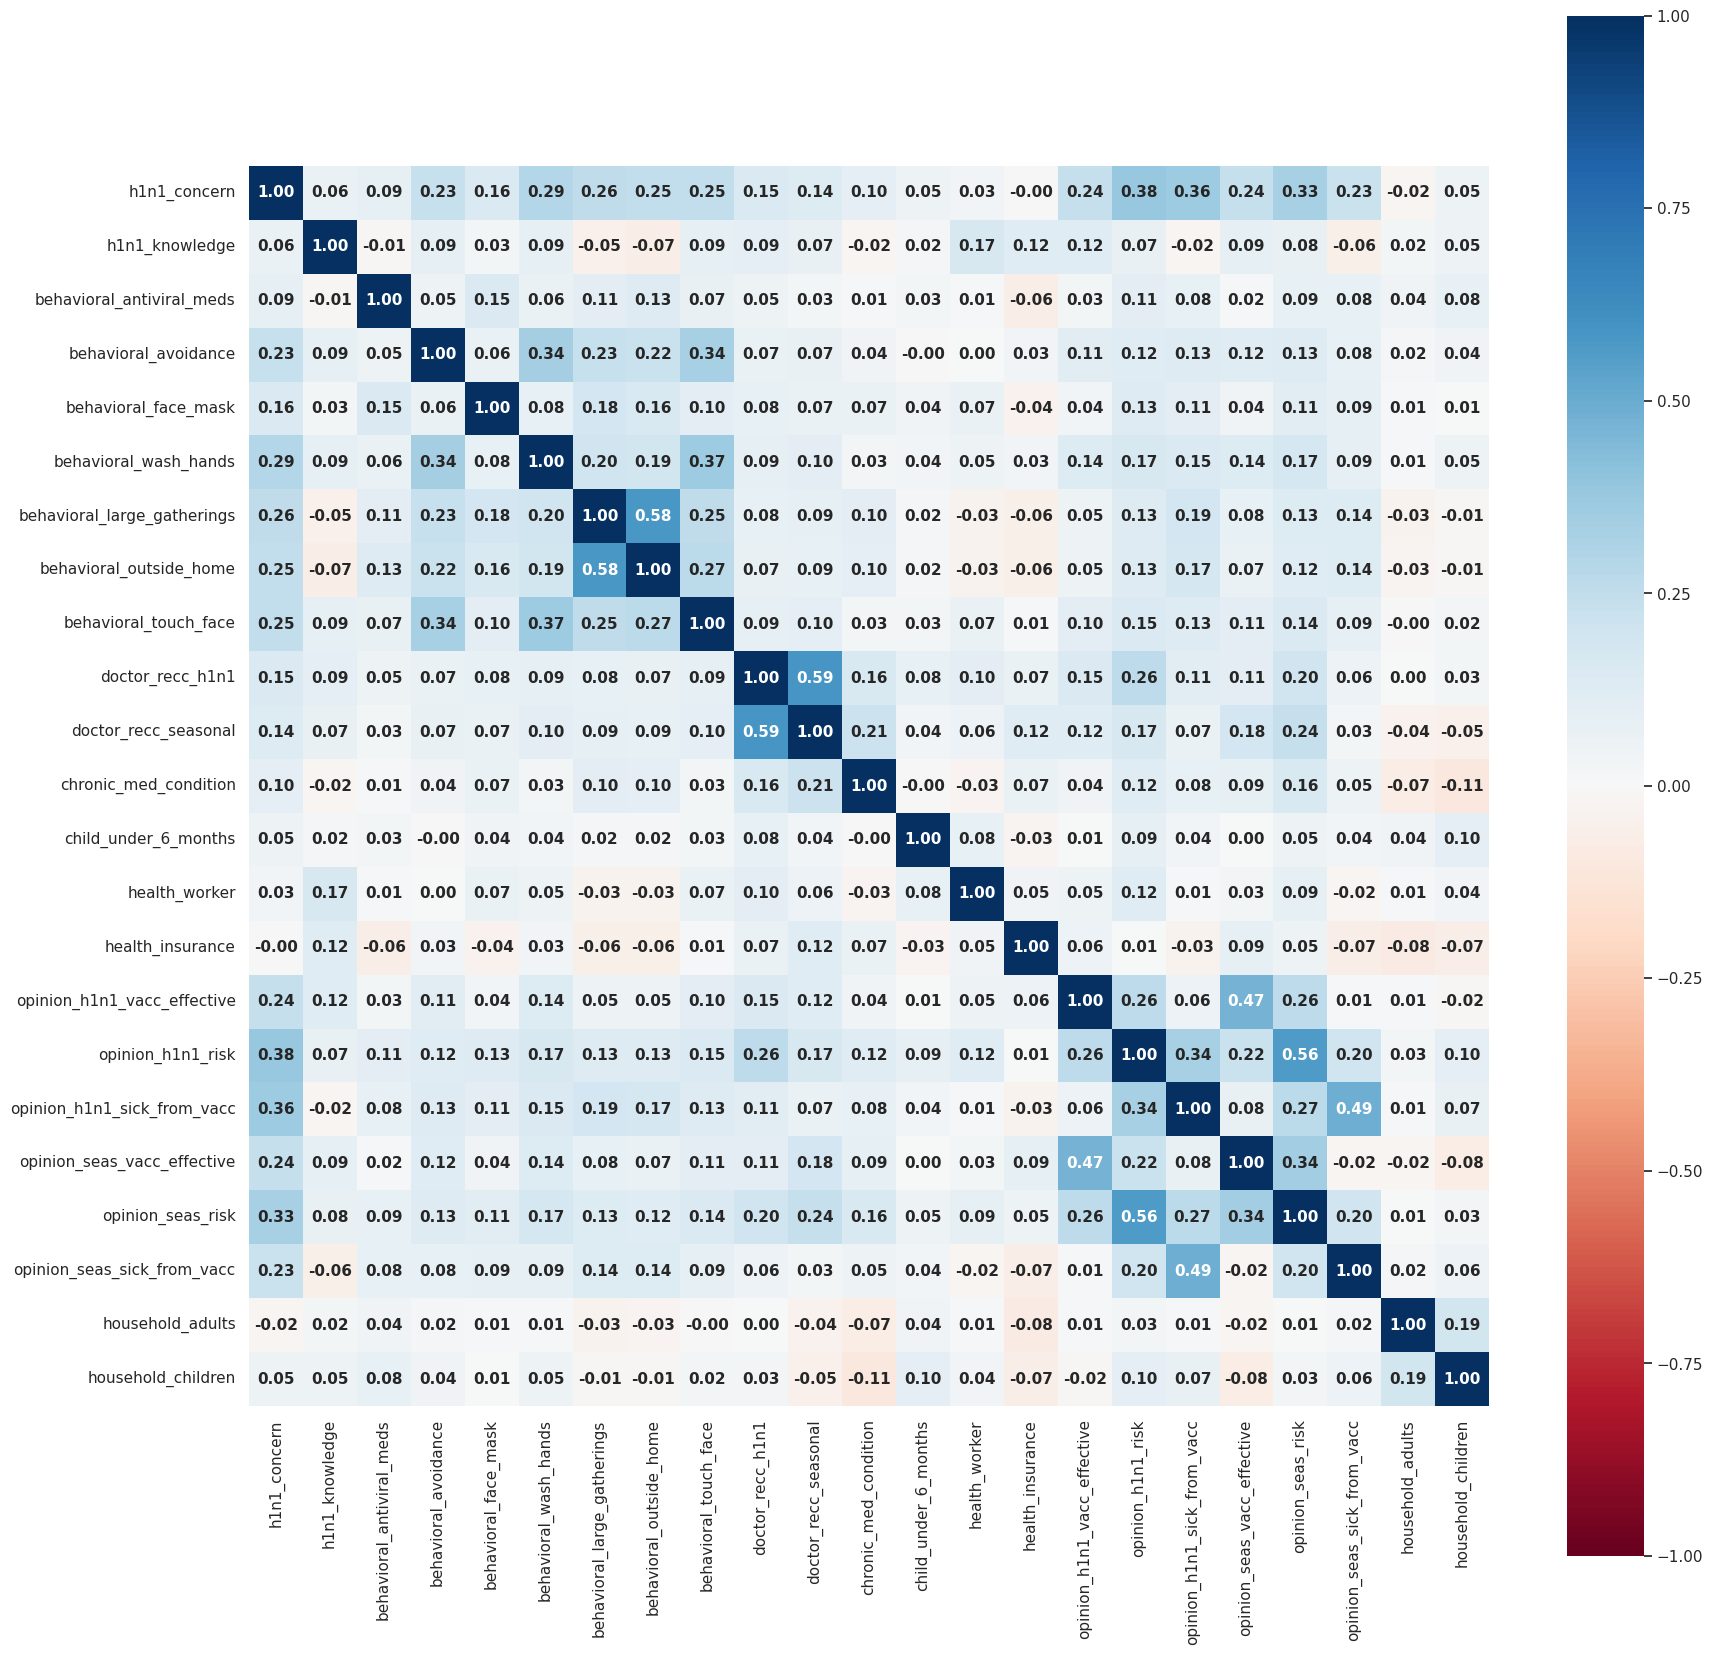
\includegraphics[width = 8cm,height=8cm]{figures/Heatmap.png}\\  
    Figure 2.1 - Feature Correlation Heatmap
\end{center}

\subsection{Class Balance and Label Correlation}
Observing the distribution of the two target variables, shown in Figure 2.2, approximately half of individuals have been vaccinated for the seasonal flu, while only 20\% have been vaccinated for H1N1. As for class balance, we can say that the distribution of individuals vaccinated for the seasonal flu is balanced, while the distribution of those vaccinated for H1N1 is imbalanced.

Taking the correlation (also known as the phi coefficient ) between the two target variables a value of approximately $\phi = 0.377$ was obtained. This indicates a positive correlation between the two target variables, meaning that these aren't fully independent from each other. 
\begin{center}
    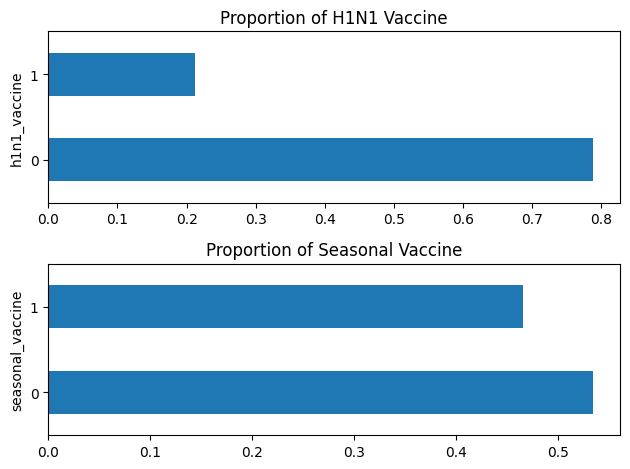
\includegraphics[width = 8cm,height=7cm]{figures/Proportion.png}\\  
    Figure 2.2 - Feature Correlation Heatmap
\end{center}



\subsection{Feature Distributions}
Firstly, it is observed that out of the people who received the seasonal vaccine, most of them were female. The same case was also observed with H1N1 vaccine through which one can conclude that women are more prone to get affected than men.
\begin{center}
    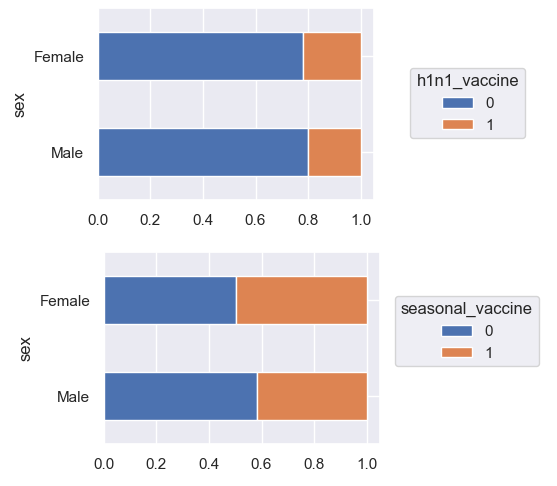
\includegraphics[width = 8cm,height=7cm]{figures/Sex.png}\\  Figure 2 - Vaccination for male and female
\end{center}

The age group has a strong correlation with the seasonal flu vaccine but not with the H1N1 flu vaccine. It seems that people act appropriately when it comes to the seasonal flu as older individuals have a higher risk of complications. However, with H1N1 flu, even though older individuals have a higher risk of complications, they are less likely to get infected. This analysis does not provide information about causality, but it seems that the risk factors are reflected in vaccination rates.
It appears that questions related to knowledge and opinions have a strong correlation with both target variables.

\begin{center}
    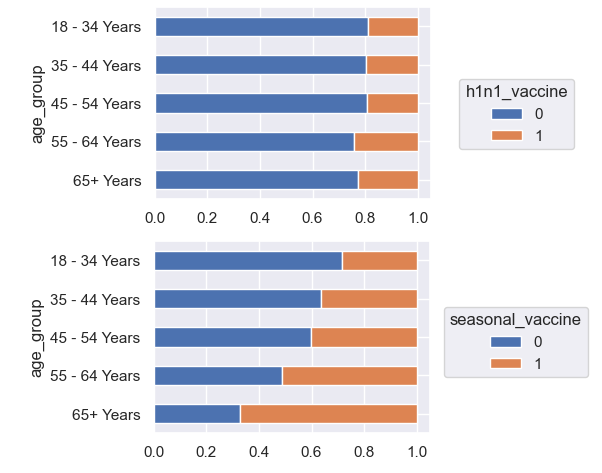
\includegraphics[width = 8cm]{figures/Age.png}\\
    Figure 2.2 - Vaccination for different age groups
\end{center}

\section{Performance Metric}
To measure the performance of the classifications performed between different classifiers, the ROC (Receiver Operating Characteristic) metric was utilized. The ROC is a type of plot used in binary classifiers, which measures the true positive rate (TPR) against the false positive rate (FPR) for different classifier thresholds. To obtain a quantitative measurement of the performance obtained, it it possible to take the area under the curve (AUC). One way of interpreting AUC is as the probability that the model ranks a random positive example more highly than a random negative example. Note that this area can be between 0 and 1, the latter characterizing a perfect classifier.
To illustrate the ROC curve, \textit{SKLearn's} \texttt{Dummy Classifier} \cite{b2} can be utilized as a random classifier, to obtain a baseline for the classifier performance. The ROC curve obtained can be seen in the graph in figure 3.1.

\begin{center}
    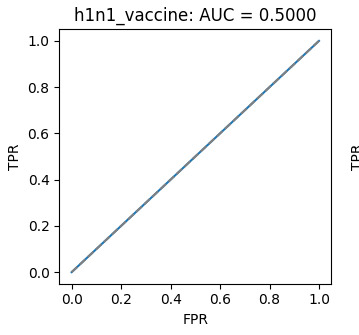
\includegraphics[width=8cm]{figures/ROC_Dummy_Classifier.png}\\
    Figure 3.1 - ROC curve for \textit{Dummy Classifier} (H1N1 vaccine)
\end{center}

If an actual classifier model is utilized, a plot like that of Figure 3.2 can be obtained. If an ideal classifier were to be used, the resulting ROC would theoretically be a single point where the TPR would be one and the FPR nil.

\begin{center}
    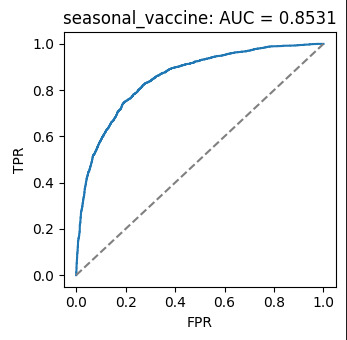
\includegraphics[width=8cm]{figures/ROC_CatBoost.png}\\
    Figure 3.2 - ROC curve for Logistic Regression (seasonal vaccine)
\end{center}

\section{Methodology}
As mentioned previously, several classification models were experimented with and compared. Some of the standard classification models utilized for the purposes of this project included Logistic Regression, Multinomial Naive Bayes, K-Nearest neighbors and Decision Trees. Besides these, two gradient boosting algorithms, \textit{CatBoost} and \textit{XGBoost} were also used.
For most of the models, in order to automate the data processing and estimation steps, \textit{SKLearn} pipelines were utilized. Within the preprocessing steps, column transformations were performed separately for the numerical and categorical features. For the numerical processing, the \texttt{StandardScaler} \textit{SKLearn}\cite{b3} class was utilized in most cases to guarantee that each column had nil mean and unit variance, followed by \texttt{SimpleImputer}\cite{b4} to fill all missing data values utilizing each columns median value.

For categorical features, missing data was also filled using \texttt{SimpleImputer}, but this time with the most frequent value, before being encoded utilizing an One-Hot Encoder, which separated each possible category within each feature into separate binary variables.
For the estimation, since most classifiers utilized did not support multi-label classification, the \texttt{MultiOutputClassifier}\cite{b5} function was utilized, which in the this case will train two separate instances of the desired estimator.

For measuring the performance of the classifiers obtained before submitting any results for the competition (only 3 daily submissions were allowed on this competition), the training set was split/folded randomly using \texttt{train\_test\_split()}\cite{b6} to obtain a performance measurement. After this, the models were trained on the entire dataset. Figure 4.1. illustrates this entire process.

\begin{center}
    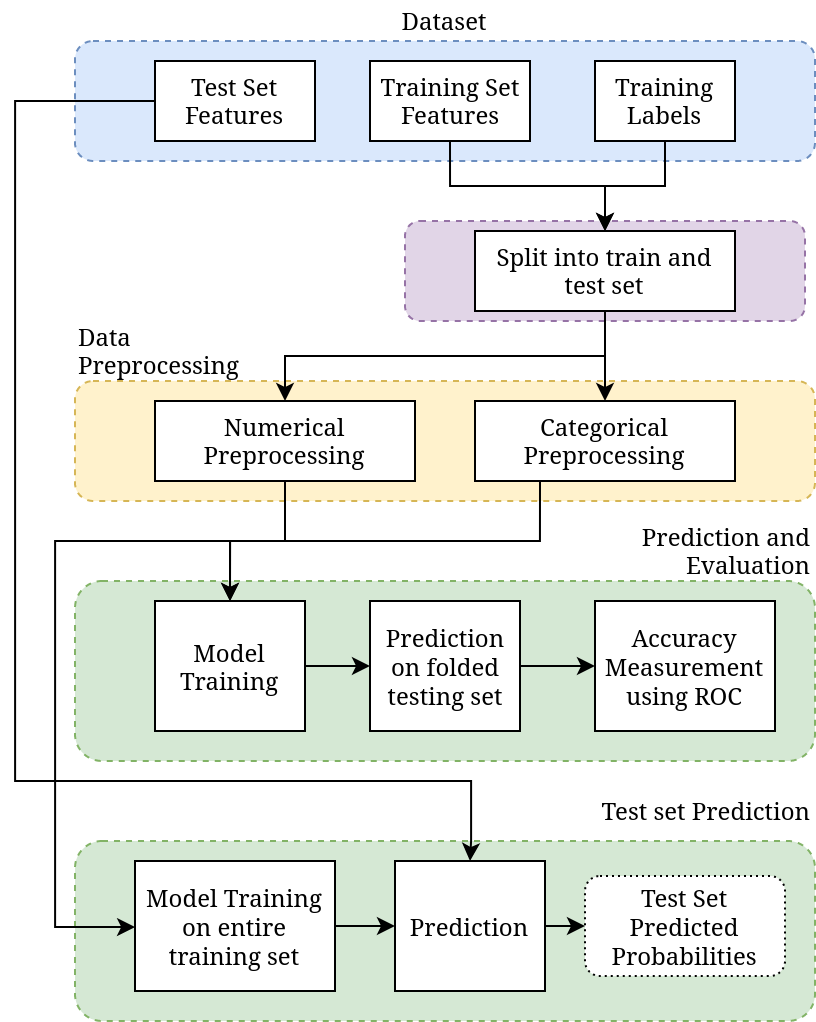
\includegraphics[width=7cm]{figures/MethodologyStructure.png}\\
    Figure 4.1 - Model Structure used
\end{center}

\subsection{Logistic Regression}
The first model to be trained was the Logistic Regression. Unlike what the name suggests, the Logistic model is a classification model rather than a regression model and is one of the most widely used techniques when it comes to solving classification problems. %\\
To utilize the Logistic Regression within our model, \textit{SKLearn} already includes an implementation of this model with the class \texttt{LogisticRegression}\cite{b7}, which includes several tweakable parameters. To iterate and compare different parameter combinations, \textit{SKLearn} includes a simple way to automate the process with the \texttt{GridSearchCV}\cite{b8} class. This was utilized for many of the models tested, and in the case of the Logistic Regression, it was utilized to figure out the optimum type of regularization and it's strength.

\subsection{Naive Bayes}

The Naive Bayes classification methods, work by applying Bayes' Theorem naively assuming that all the features are conditionally independent from each other. The prior and posterior can then be estimated in different ways.

\textit{SKLearn} includes several Naive Bayes based classifiers, of which the \texttt{GaussianNB}\cite{b9} and \texttt{MultinomialNB}\cite{b10} were utilized in this project. \texttt{GaussianNB} assumes that the likelihood of each feature given the label is a gaussian function. Meanwhile, \texttt{MultinomialNB} assumes that the data is multinomially distributed, and as such it estimates the posterior probabilities by counting how often a given value appears within each label, for each feature. While using the multinomial model, it was required to remove the standardization/scaling that was applied to the numerical features.

\subsection{K-Nearest Neighbors}

The K-Nearest Neighbors is a machine learning algorithm that can be used for both regression and classification. In the case of classification, the algorithm computes the $k$ closest neighbors to the observation, and classifies the observation based on what class held the majority among those neighbors.

This method can achieve very good results depending on what value of $k$ is utilized. A larger k will generally suppress the effect of noise on the data, but makes the decision boundary less clear which might affect the ROC score. To use the model, \textit{SKLearn} includes the \texttt{KNeighborsClassifier} \cite{b11} class, which was used in combination with \texttt{GridSearchCV} to find the value $k$ that produces the best results.

\subsection{Decision Trees}

Decision Trees are models that attempt to match the target variable by learning decisions from the training data and applying these decisions to the features of an observation's features. These models have the advantage of being conceptually easy to understand, but are quite prone to overfitting the training data.

Similarly to the previous models, the \textit{SKLearn} implementation of the decisions trees, \texttt{DecisionTreeClassifier} \cite{b12}, was utilized.

\subsection{XGBoost}

\textit{XGBoost} (which stands for eXtreme Gradient Boosting), is a library that provides many gradient boosting algorithms \cite{b13}. Essentially, gradient boosting gives a result based on an ensemble of many weaker learning models, as for example decision trees, combining these sequentially and having each stage correct the errors of the previous one.

This library provides many different models and several interfaces for different programming environments. For the purposes of this work, the \texttt{XGBClassifier} class was used, as it easily integrates with the \textit{SKLearn}.

\subsection{CatBoost}

The final model that was utilized in this project was \textit{CatBoost}. Similarly to XGBoost, and as the name implies, \textit{CatBoost} is also a gradient boosting library. The advantage of \textit{CatBoost} is that it natively supports categorical features without any need for encoding these. This library provides a classification model, also compatible with \textit{SKLearn}, through the class \texttt{CatBoostClassifier} \cite{b14}.

This model was utilized in two ways, firstly by integrating it into the pipeline developed previously (in the notebook \texttt{Project\_mainModel.ipynb}, including categorical feature encoding) and in a separate preprocessing pipeline in the file \texttt{Project\_catBoostedModel.ipynb}. This was done since the first the pipeline utilized \textit{SKLearn's} ColumnTransformers, which made it challenging to specify what columns were categorical in \textit{CatBoost}.

\section{Results}

\subsection{Result Analysis}

Examining the experimental results for all the non gradient boosting models, the following results were obtained:

\begin{center}
    \begin{tabular}{|l|l|}
        \hline
    \textbf{Model} & \textbf{ROC AUC score} \\ 
    \hline \hline
    Logistic regression (C = 0.01) & 0.84555 \\ \hline
    Logistic regression (C = 0.1) & 0.84655 \\ \hline
    Logistic regression (C = 1) & 0.84640 \\ \hline
    Logistic regression (C = 10) & 0.84635 \\ \hline
    Gaussian Naive Bayes & 0.72947 \\ \hline
    Multinomial Naive Bayes & 0.79467 \\ \hline
    Decision Tree & 0.66738 \\ \hline
    KNearestNeighbors (k=169) & 0.82478 \\ \hline
    \end{tabular}\\
    \vspace{7pt}
    Table 5.1 - Scores for some of the models tested
\end{center}

It is possible to see that all the Logistic Regression models exhibited the best classification performance, having pretty much the same score for all the values of C. This parameter is essentially the inverse of the regularization strength. 
The worst performing model out of all, was clearly the Decision tree classifier. Observing the ROC plot for the Decision Tree, shown in figure 5.1, it is possible to see that it is composed of two straight lines, due to this classifier not being able to estimate the probability of each label, but instead assigning an hard label to each observation.

\begin{center}
    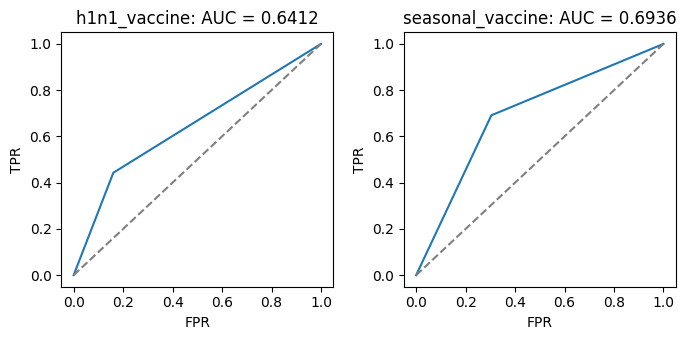
\includegraphics[width=8cm]{figures/decisionTreeROC.png}\\
    Figure 5.1 - ROC plot for the Decision Tree classifier
\end{center}

In terms of the Naive Bayes classifiers, it is possible to see that the multinomial distribution approximation presents much promising results than the Gaussian approximation.

Taking a look at the results K-Nearest Neighbors, first the score plot of Figure 5.2 was obtained by varying the number of neighbors used and averaging the score across 10 folds of the dataset. It is possible to observe that above a certain threshold of k, that the score seems to stagnate.

\begin{center}
    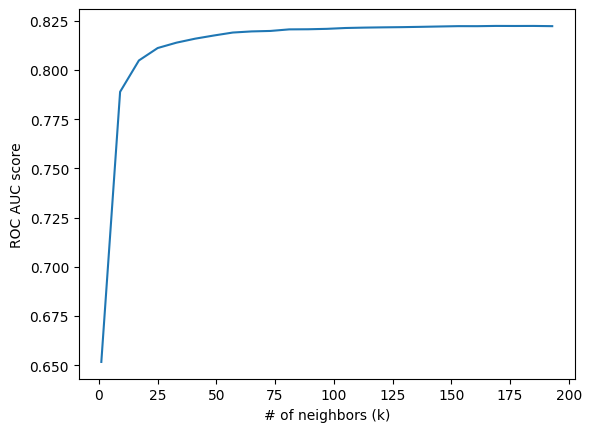
\includegraphics[width=8cm]{figures/KNN_score.png}\\
    Figure 5.2 - K-Nearest Neighbors ROC AUC Score for varying number of neighbors
\end{center}

As for the gradient boosting models, the results were the following:

\begin{center}
    \begin{tabular}{|l|l|}
        \hline
    \textbf{Model} & \textbf{ROC AUC score} \\ 
    \hline \hline
    XGBoost (Default parameters) & 0.83732 \\ \hline
    CatBoost with One-Hot encoding & 0.85069 \\ \hline
    CatBoost with specified cat\_features & 0.86907 \\ \hline
    \end{tabular}\\
    
    \vspace{6pt}
    Table 5.2 - Scores for the gradient boosting models
\end{center}

It is possible to see that \textit{CatBoost} performs much better than \textit{XGBoost}, which itself performed worse than the Logistic Regression models used initially. These results also make it evident that to achieve the full potential of \textit{CatBoost}, there isn't much preprocessing needed, only simple imputation and categorical column identification is needed.

\subsection{Competition Results}

Applying the unseen competition test data to some of the best performing models, the following results were obtained:

\begin{center}
    \begin{tabular}{|l|l|}
        \hline
    \textbf{Model} & \textbf{ROC AUC score} \\ 
    \hline \hline
    Logistic Regression (C=0.1) & 0.8356 \\ \hline
    K-Nearest Neighbors (k=169) & 0.8122 \\ \hline
    CatBoost with One-Hot encoding & 0.8430 \\ \hline
    CatBoost with specified cat\_features & 0.8616 \\ \hline
    \end{tabular}\\
    
    \vspace{6pt}
    Table 5.3 - Scores obtained during the competition submissions
\end{center}

With these results, it was very clear that \textit{CatBoost} demonstrated exceptional performance when compared to every other model tested. The final score of 0.8616 granted our team the 285th position on this competition's leaderboard. The top submission at the time of writing is a 0.8658, meaning that our classifier's performance is within 0.5\% of the top 1 result.

\section{Conclusion}

From this project, it can be concluded that the design process of a classification model, even if using existing implementations, is a fundamental part of many machine learning applications and that knowing the nuances of this is essential in order to design good performing machine learning models. This project also gave insight to the characterization of binary classifiers, specifically using the Receiver Operating Characteristic metric. 

The performance could have possibly been improved if an alternative to the \texttt{MultiOutputClassifier} had been used, since this class creates two separate classifiers, regardless of any possible relation between labels. Still, the results obtained using \textit{CatBoost} were very promising.

Overall, it can be said that all the objectives set for this project were met, and that further knowledge of the concepts studied here has been obtained.

\begin{thebibliography}{00}
    \bibitem{b1} DrivenData, “Flu shot learning: Predict H1N1 and seasonal flu vaccines,” DrivenData. [Online]. Available: \url{https://www.drivendata.org/competitions/66/flu-shot-learning/}. [Accessed: 09-Jan-2023].
    \bibitem{b2} “Sklearn.dummy.DummyClassifier,” scikit. [Online]. Available: \url{https://scikit-learn.org/stable/modules/generated/sklearn.dummy.DummyClassifier.html}. [Accessed: 10-Jan-2023].

    \bibitem{b3} “Sklearn.preprocessing.StandardScaler,” scikit. [Online]. Available: \url{https://scikit-learn.org/stable/modules/generated/sklearn.preprocessing.StandardScaler.html}. [Accessed: 10-Jan-2023]. 

    \bibitem{b4} “Sklearn.impute.SimpleImputer,” scikit. [Online]. Available: \url{https://scikit-learn.org/stable/modules/generated/sklearn.impute.SimpleImputer.html}. [Accessed: 10-Jan-2023].

    \bibitem{b5} “Sklearn.multioutput.multioutputclassifier,” scikit. [Online]. Available: \url{https://scikit-learn.org/stable/modules/generated/sklearn.multioutput.MultiOutputClassifier.html}. [Accessed: 10-Jan-2023]. 

    \bibitem{b6} “Sklearn.model\_selection.train\_test\_split,” scikit. [Online]. Available: \url{https://scikit-learn.org/stable/modules/generated/sklearn.model_selection.train_test_split.html}. [Accessed: 10-Jan-2023].

    \bibitem{b7} “Sklearn.linear\_model.logisticregression,” scikit. [Online]. Available: \url{https://scikit-learn.org/stable/modules/generated/sklearn.linear_model.LogisticRegression.html}. [Accessed: 10-Jan-2023]. 

    \bibitem{b8} “Sklearn.model\_selection.GRIDSEARCHCV,” scikit. [Online]. Available: \url{https://scikit-learn.org/stable/modules/generated/sklearn.model_selection.GridSearchCV.html}. [Accessed: 10-Jan-2023]. 

    \bibitem{b9} “Sklearn.naive\_bayes.Gaussiannb,” scikit. [Online]. Available: \url{https://scikit-learn.org/stable/modules/generated/sklearn.naive_bayes.GaussianNB.html}. [Accessed: 10-Jan-2023]. 

    \bibitem{b10} “Sklearn.naive\_bayes.multinomialnb,” scikit. [Online]. Available: \url{https://scikit-learn.org/stable/modules/generated/sklearn.naive_bayes.MultinomialNB.html}. [Accessed: 10-Jan-2023]. 

    \bibitem{b11} “Sklearn.neighbors.kneighborsclassifier,” scikit. [Online]. Available: \url{https://scikit-learn.org/stable/modules/generated/sklearn.neighbors.KNeighborsClassifier.html}. [Accessed: 10-Jan-2023]. 

    \bibitem{b12} “Sklearn.tree.decisiontreeclassifier,” scikit. [Online]. Available: \url{https://scikit-learn.org/stable/modules/generated/sklearn.tree.DecisionTreeClassifier.html}. [Accessed: 12-Jan-2023].

    \bibitem{b13} “XGBoost documentation,” XGBoost Documentation - xgboost 1.7.3 documentation. [Online]. Available: \url{https://xgboost.readthedocs.io/en/stable/}. [Accessed: 12-Jan-2023].

    \bibitem{b14} “Catboostclassifier,” CatBoost. [Online]. Available: \url{https://catboost.ai/en/docs/concepts/python-reference_catboostclassifier}. [Accessed: 15-Jan-2023]. 
\end{thebibliography}

\end{document}
